\chapter{RESULTADOS E DISCUSS\~AO}
\label{cap:capitulo4}

\section{Desempenho dos modelos}
%Apresentar e comparar os resultados dos diferentes modelos utilizados.

Os resultados obtidos pelos modelos variaram significativamente em termos de precisão, tanto nas previsões pontuais quanto nos intervalos de previsão, refletindo diferentes graus para cada cenário analisado. Observar o comportamento dos resíduos foi interessante pois dependendo da época do ano, houve um comportamento bastante destacado.

\subsection{Rio Jequitinhonha}

Começando pela menor bacia estudada, os resultados mostraram-se bastante satisfatórios, especialmente no que tange à Regressão Linear, que se destacou com boas previsões tanto em termos pontuais quanto nos intervalos de previsão. Este modelo demonstrou uma boa capacidade de capturar a dinâmica hidrológica do rio, refletindo precisão nas métricas e um desempenho consistente. E com um tempo de execução muito baixo. O modelo simples \textit{SeasonalNaive} apresentou resultados aquém do esperado em todas as situações avaliadas, considerando a previsão pontual e os intervalos de previsão.

Com um MAPE muito elevado de 150\%, o resultado mostrou viés de superestimação dos resultados, conforme a métrica PBIAS aponta. Olhando para a qualidade dos intervalos de previsão pode-se acreditar que o modelo teve um comportamento satisfatório, contudo, com mais atenção, é possível ver que o valor inferior do intervalo (lo-95) foram calculados números abaixo de zero. O atraso (\textit{delay}) da série prevista foi de elevados 56,88 dias, com um desvio-padrão de 61,3 dias, de onde se observa que um evento pode levar mais de 60 dias para ser percebido na previsão do modelo.

Como o modelo SN a análise termina aqui, não se procedeu com análise de resíduos nem com importância de variáveis uma vez que o desempenho do modelo foi ruim. Está aqui para comparação. A análise mais aprofundada mesmo ficará por conta dos modelos mais complexos.

\begin{figure}[!h]
	\centering
	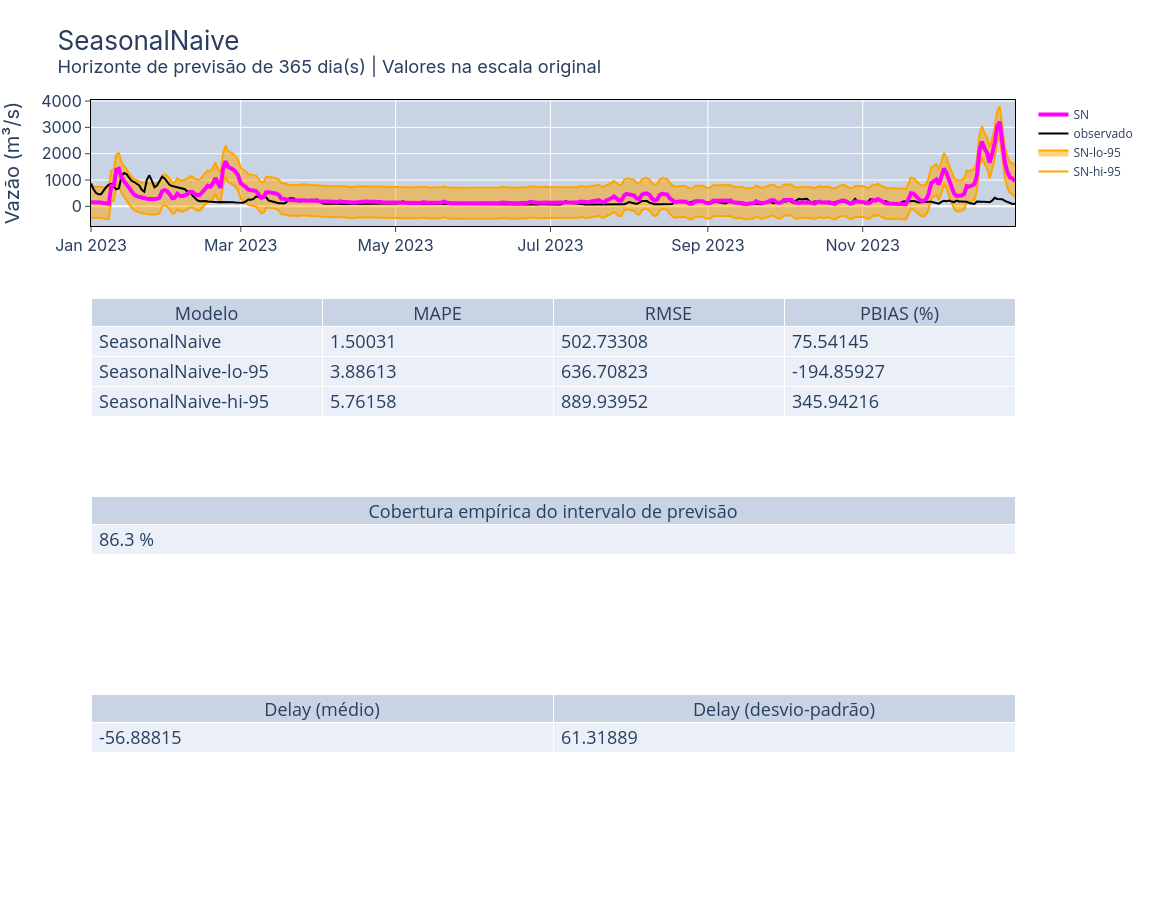
\includegraphics[scale=0.33]{Figuras/jequiti/resultados/SN_WFV.png}
	\caption{Resultado do SeasonalNaive no teste \textit{Walk-Forward Validation}\\(fonte: o autor)}
	\label{fig:jequiti_SN_WFV}
\end{figure}

%\begin{table}[!h]
%	\centering \small
%	\caption{Resultados SeasonalNaive - rio Jequitinhonha \\(fonte: o autor)}
%	\begin{tabular}{|l|r|r|r|r|r|r|} \hline 
	%		\textbf{Horizonte} & \textbf{MAPE} & \textbf{RMSE} & \textbf{PBIAS} \\\hline
	%		1 dia              & 0,871         & 831,44        & -87,11 \\\hline
	%		3 dias             & 1,528         & 1872,25       & 102,71 \\\hline
	%		7 dias             & 1,046         & 1529,13       & 49,64  \\\hline
	%		15 dias            & 0,791         & 1468,02       & -13,46 \\\hline
	%	\end{tabular}
%	\label{tab:sn_jequitinhonha_resultados}
%\end{table}

Os resultados obtidos utilizando o modelo de Regressão Linear mostraram-se bastante promissores.

\begin{figure}[!h]
	\centering
	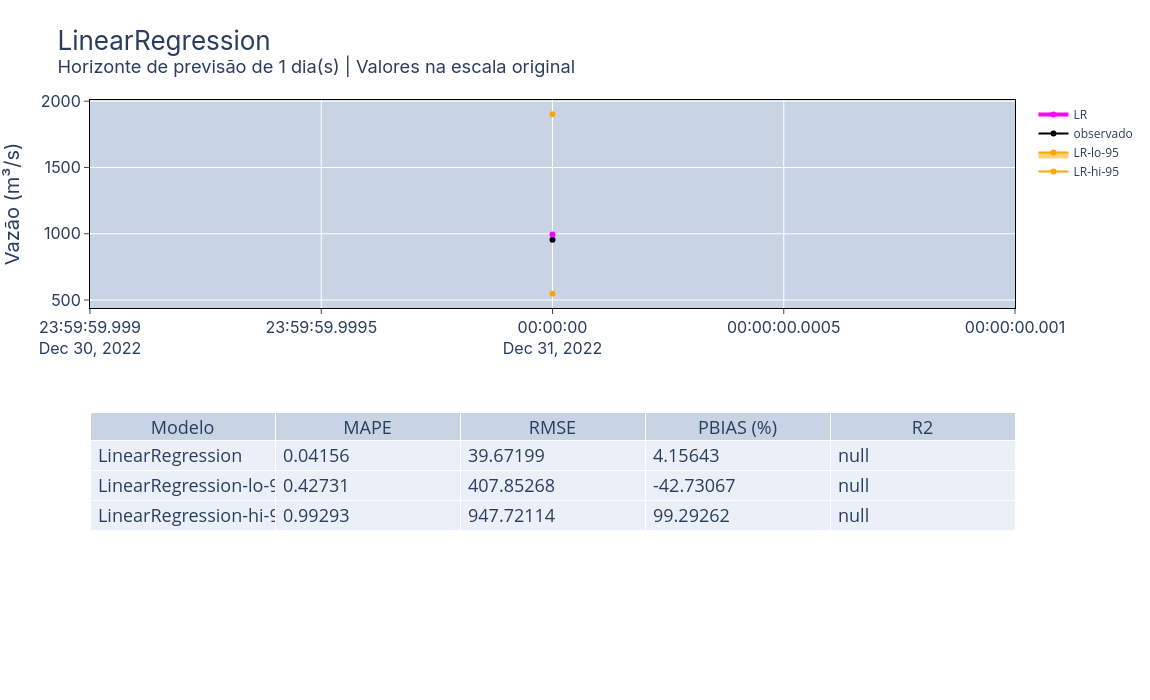
\includegraphics[scale=0.33]{Figuras/jequiti/resultados/LinearRegression_fh1.png}
	\caption{Regressão Linear para o horizonte de previsão de 1 dia\\(fonte: o autor)}
	\label{fig:jequiti_LinearRegression_fh1}
\end{figure}

Continuando a análise, agora os modelos principais do trabalho, ajustados com variáveis categóricas para melhor realizar as previsões a partir da sazonalidade.

Houve uma intercalação no desempenho dos resultados. Para o horizonte de 1 dia, o RandomForest apresentou um resultado melhor em relação ao CatBoost em todas as métricas. O intervalo de previsão também foi melhor pois capturou o valor observado, coisa que o CatBoost não fez.(figuras \ref{fig:jequiti_RandomForest_fh1} e \ref{fig:jequiti_CatBoostRegressor_fh1})

Quando aumentou o horizonte para 3 dias, o CatBoost apresentou melhor desempenho, inclusive nos intervalos de previsão.(figura \ref{fig:jequiti_CatBoostRegressor_fh3})

\begin{figure}[!h]
	\centering
	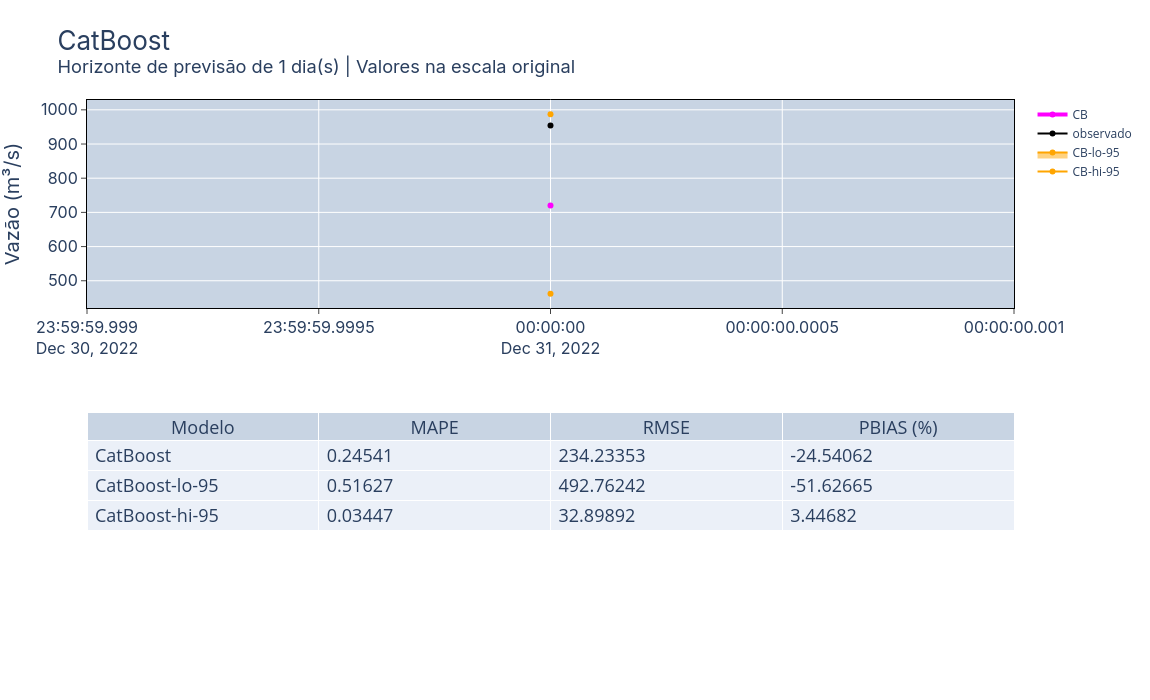
\includegraphics[scale=0.33]{Figuras/jequiti/resultados/CatBoost_fh1.png}
	\caption{CatBoost para o horizonte de previsão de 1 dia\\(fonte: o autor)}
	\label{fig:jequiti_CatBoostRegressor_fh1}
\end{figure}

\begin{figure}[!h]
	\centering
	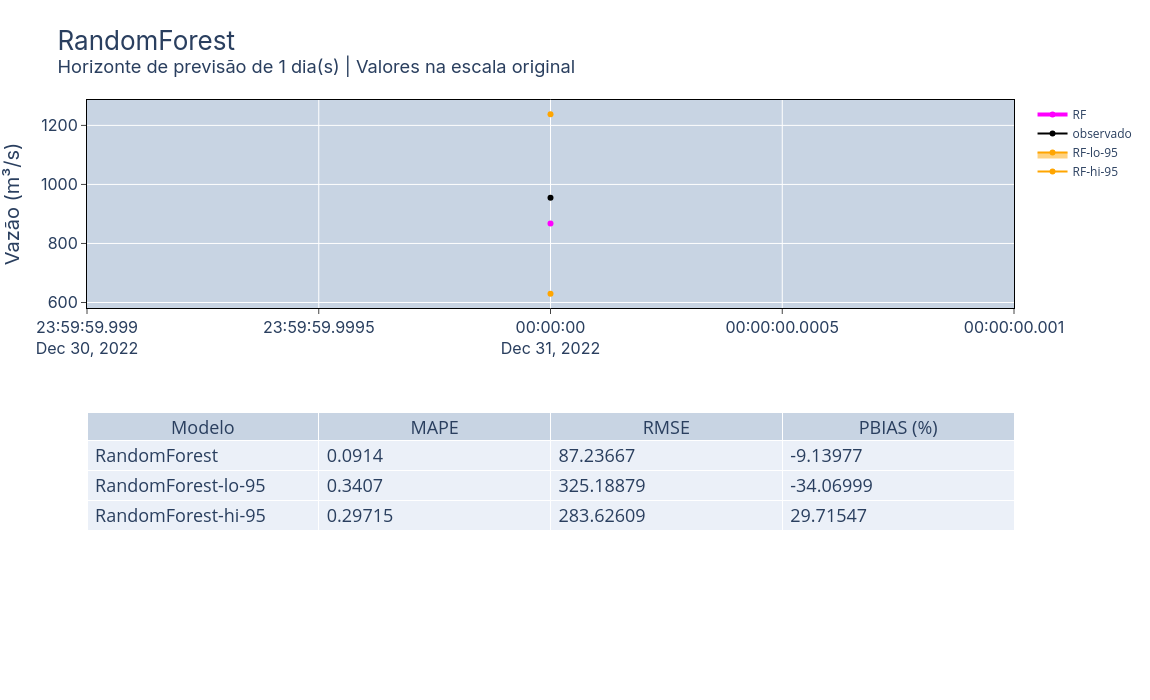
\includegraphics[scale=0.33]{Figuras/jequiti/resultados/RandomForest_fh1.png}
	\caption{RandomForest para o horizonte de previsão de 1 dia\\(fonte: o autor)}
	\label{fig:jequiti_RandomForest_fh1}
\end{figure}

\begin{figure}[!h]
	\centering
	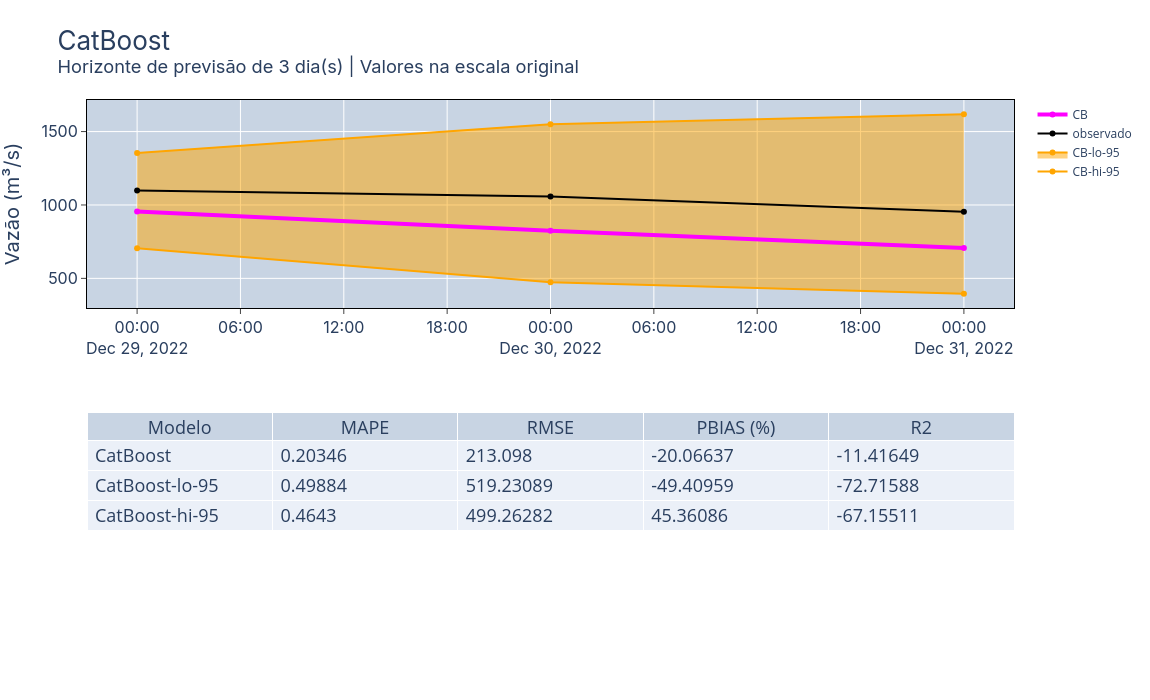
\includegraphics[scale=0.33]{Figuras/jequiti/resultados/CatBoost_fh3.png}
	\caption{CatBoost para o horizonte de previsão de 3 dias\\(fonte: o autor)}
	\label{fig:jequiti_CatBoostRegressor_fh3}
\end{figure}

\begin{figure}[!h]
	\centering
	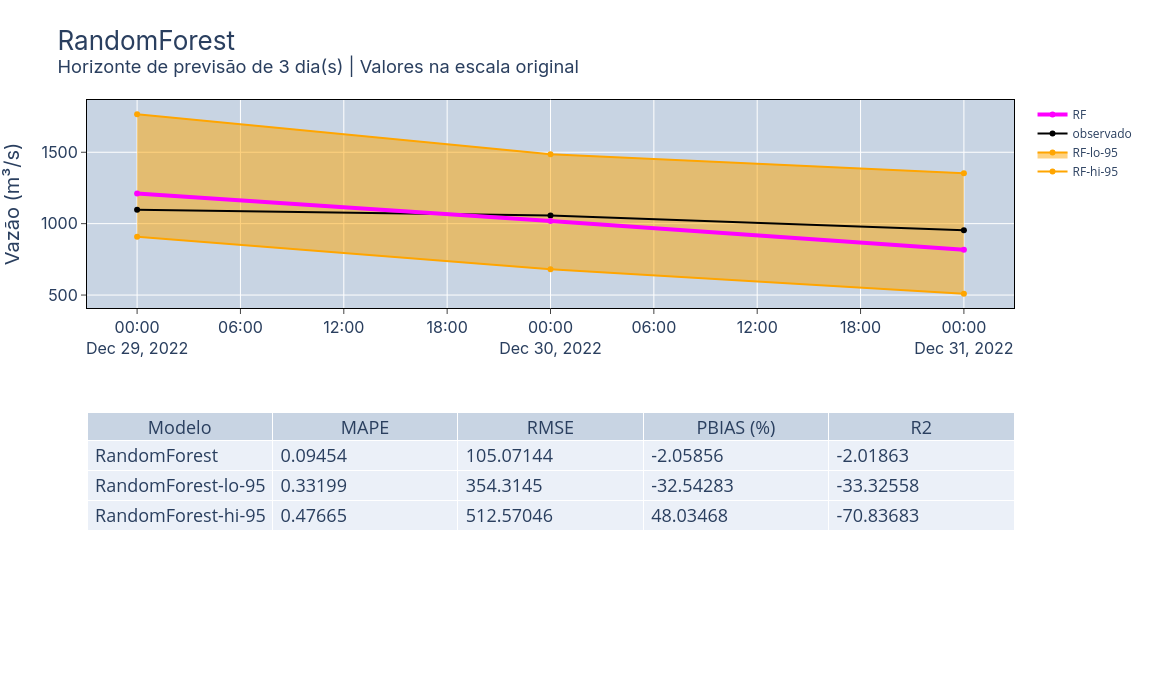
\includegraphics[scale=0.33]{Figuras/jequiti/resultados/RandomForest_fh3.png}
	\caption{RandomForest para o horizonte de previsão de 3 dias\\(fonte: o autor)}
	\label{fig:jequiti_RandomForest_fh3}
\end{figure}

\begin{figure}[!h]
	\centering
	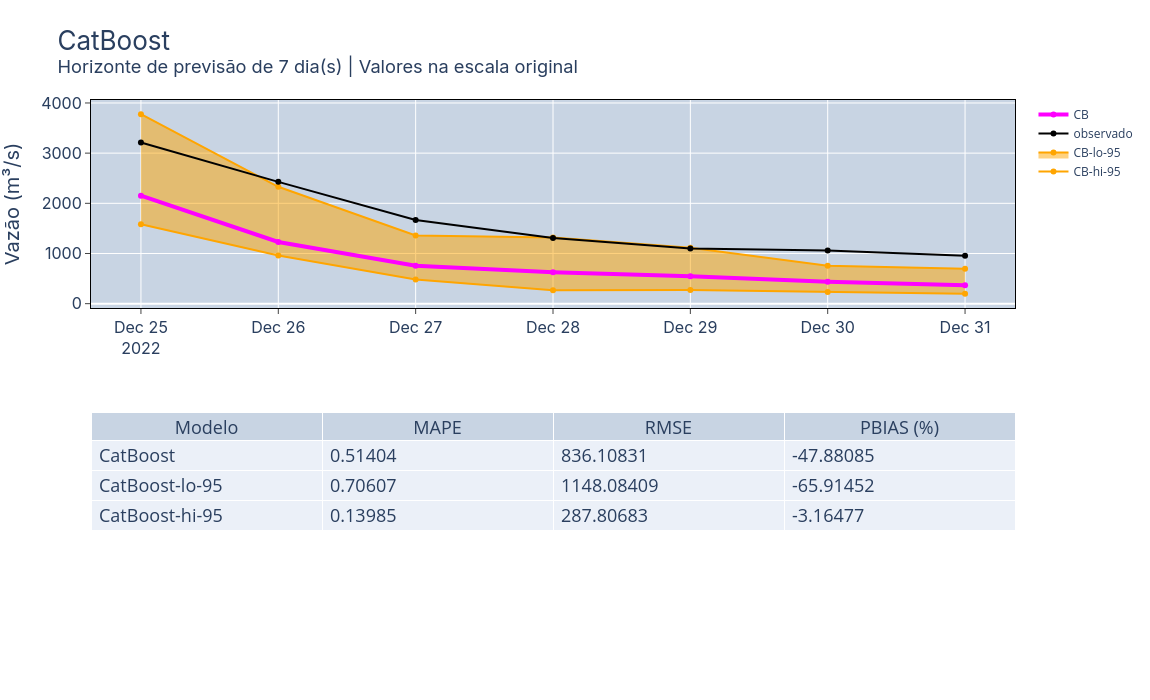
\includegraphics[scale=0.33]{Figuras/jequiti/resultados/CatBoost_fh7.png}
	\caption{CatBoost para o horizonte de previsão de 7 dias\\(fonte: o autor)}
	\label{fig:jequiti_CatBoostRegressor_fh7}
\end{figure}

\begin{figure}[!h]
	\centering
	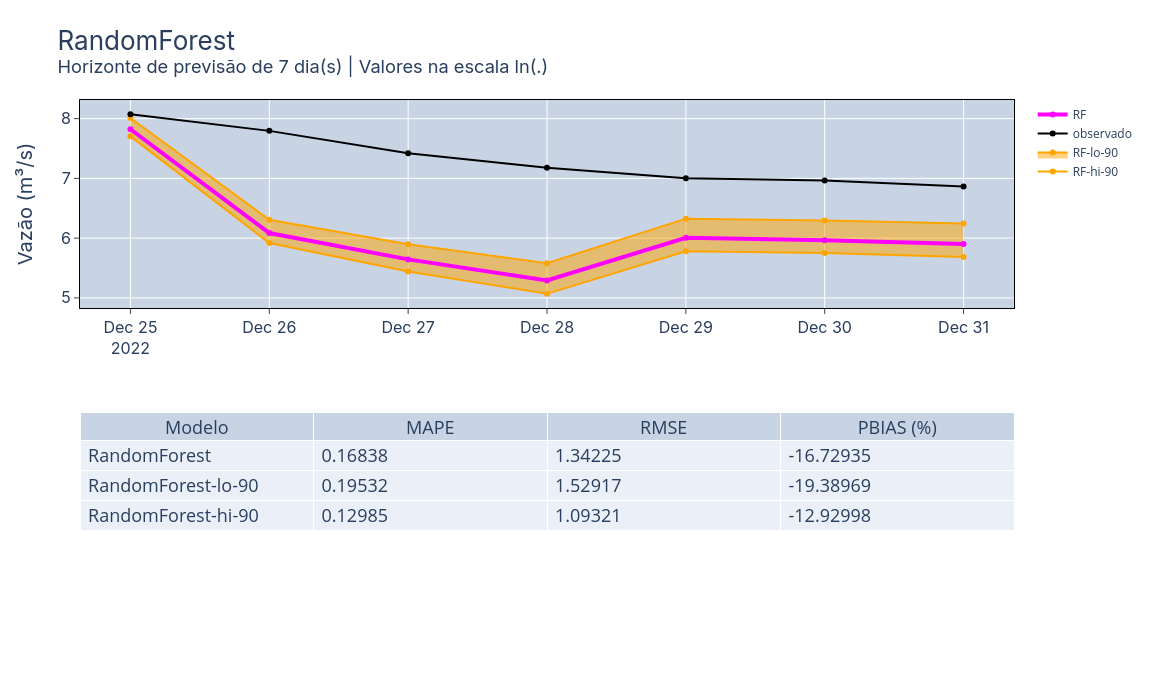
\includegraphics[scale=0.33]{Figuras/jequiti/resultados/RandomForest_fh7.png}
	\caption{RandomForest para o horizonte de previsão de 7 dias\\(fonte: o autor)}
	\label{fig:jequiti_RandomForest_fh7}
\end{figure}

\begin{figure}[!h]
	\centering
	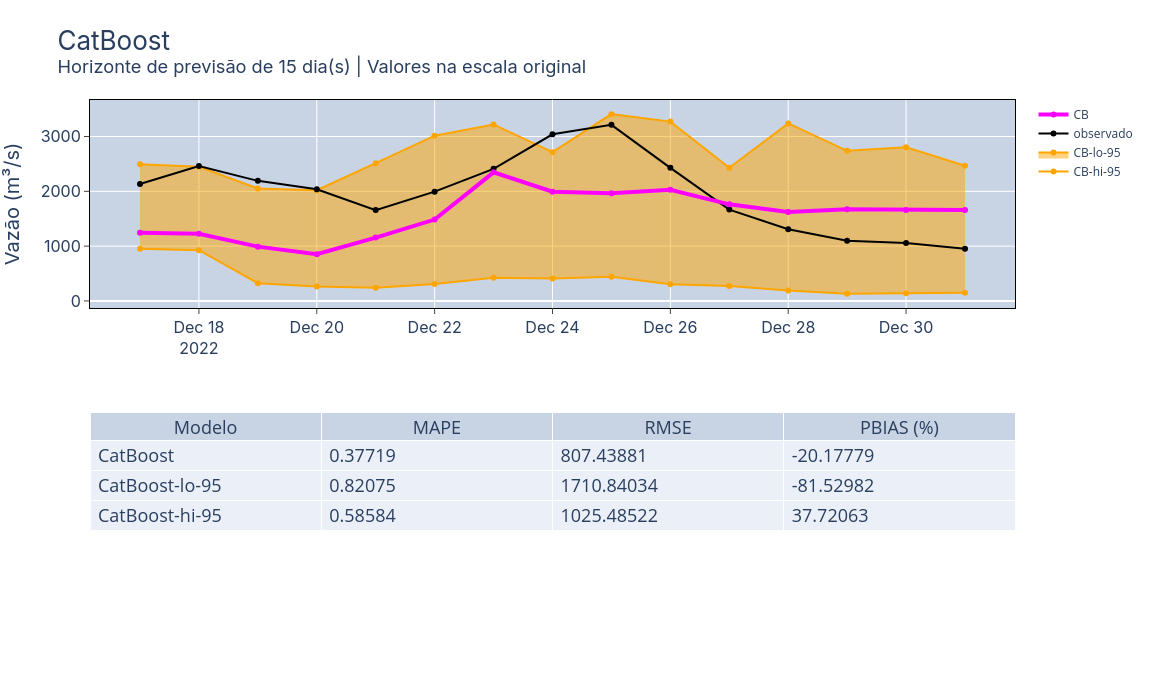
\includegraphics[scale=0.33]{Figuras/jequiti/resultados/CatBoost_fh15.png}
	\caption{CatBoost para o horizonte de previsão de 15 dias\\(fonte: o autor)}
	\label{fig:jequiti_CatBoostRegressor_fh15}
\end{figure}

\begin{figure}[!h]
	\centering
	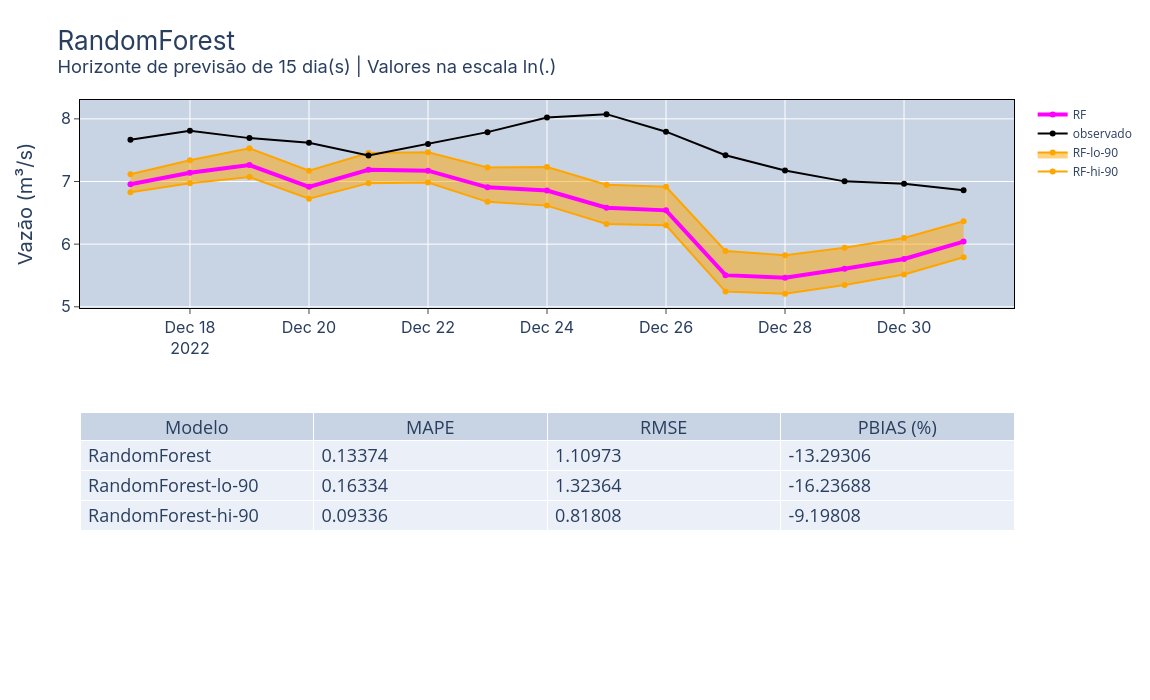
\includegraphics[scale=0.33]{Figuras/jequiti/resultados/RandomForest_fh15.png}
	\caption{RandomForest para o horizonte de previsão de 15 dias\\(fonte: o autor)}
	\label{fig:jequiti_RandomForest_fh15}
\end{figure}
\clearpage

\section{Importância das variáveis}
%Analisar a importância das variáveis contínuas e categóricas na previsão (feature importance).

\section{Discuss\~ao dos resultados}
%Interpretar os resultados e discutir as limitações. Se possível, comparar com estudos anteriores.